\section{Durchf\"uhrung}

\subsection{Versuchsanordnung}

Der Laser  wurde eingeschaltet und  der Umlenkspiegel wurde so  angepasst, bis
der Laserstrahl parallel zur langen Tischkante verlaufte, was in der Abbildung
\ref{fig:laser-angle} links  ersichtlich ist. Weiter wurde die  H\"ohe $h$ vom
Laser zum Tisch gemessen und der  Strahl nach dem Umlenkspiegel an die gleiche
h\"ohe $h$  angepasst, was in der  Abbildung \ref{fig:laser-angle} illustriert
ist.

\begin{figure}[H]
    \center
    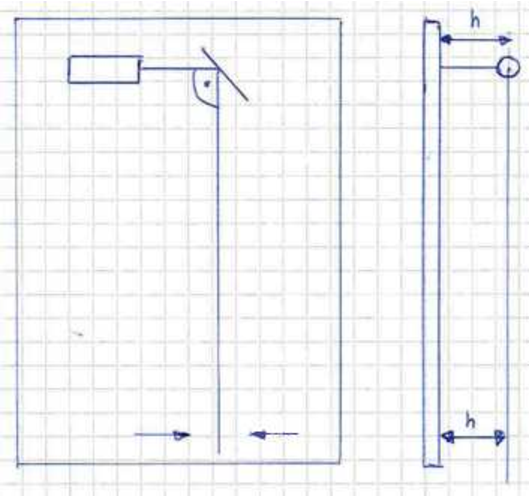
\includegraphics[width=.5\textwidth]{images/laser-angle.pdf}
    \caption{}
    \label{fig:laser-angle}
\end{figure}

Der  Laser und  der Hohlspiegel  $HS$  befinden sich  auf separate  Tische. Die
H\"ohen der Tische zum Boden $h_3$ und $h_4$ wurden gemessen. Die H\"ohe $h_2$
-- also  die Distanz  zwischen dem  Zentrum des Hohlspiegels  und dem  Tisch --
wurde weiter durch  Feinjustieren des Umlenkspiegels angepasst  bis $h_1+h_3 =
h_2+h_4$.

\begin{figure}[H]
    \center
    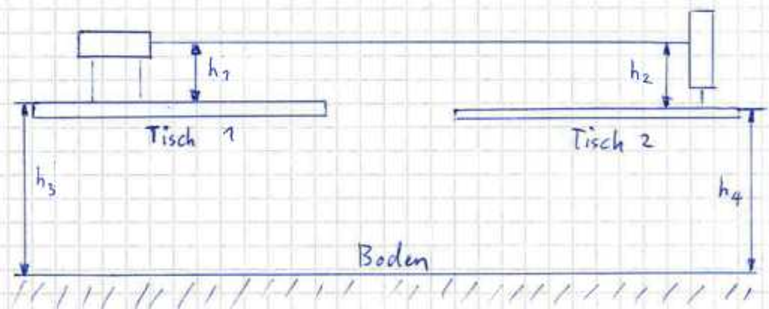
\includegraphics[width=.8\textwidth]{images/laser-height.pdf}
    \caption{}
    \label{fig:laser-height}
\end{figure}

Die gemessene H\"ohen betrugen nach der Anpassung

\begin{tabular}{ll}
    \hspace{4mm}
    & $h_1 = (\bar{h}_1 \pm s_{\bar{h}_1}) = (256\pm3)\textrm{mm}$ \\
    & $h_2 = (\bar{h}_2 \pm s_{\bar{h}_2}) = (265\pm3)\textrm{mm}$ \\
    & $h_3 = (\bar{h}_3 \pm s_{\bar{h}_3}) = (904\pm1)\textrm{mm}$ \\
    & $h_4 = (\bar{h}_4 \pm s_{\bar{h}_4}) = (895\pm1)\textrm{mm}$ \\
\end{tabular}

In der Abbildung \ref{fig:setup} ist eine Skizze der Messeinrichtung.

Der  Umlenkspiegel  $US$  wird  nun  in  den  Laserstrahl  platziert  und  auf
den  Zentrum  des Drehspiegels  $DS$  ausgerichtet.   Durch Feinjustieren  des
Umlenkspiegels  $US$   kann  der  Laserstrahl   genau  auf  den   Zentrum  des
Drehspiegels $DS$ ausgerichtet werden.

Der  Motor des  Drehspiegels wird  von Hand  rotiert bis  der Drehspiegel  den
Laserstrahl genau auf den Zentrum des Hohlspiegels $HS$ umlenkt.

Nun  wird  der  Hohlspiegel  $HS$  angepasst  und  feinjustiert,  bis  er  den
Strahl auf  dem Zentrum  des Endspiegels $ES$  umlenkt. Dabei ist  es wichtig,
dass  die  Distanz   zwischen  den  Spiegeln  $HS$  und  $ES$   genau  $f_2  =
(4985\pm5)\textrm{mm}$ betr\"agt. Der Endspiegel $ES$ wurde verschoben und mit
einem  Laserdistanzmessger\"at wurde  die Distanz  auf $(4.988\pm3)\textrm{m}$
gemessen.

Nun  wird  der  Endspiegel  $ES$  feinjustiert,  bis  der  Laserstrahl  wieder
direkt  auf  den Hohlspiegel  $HS$  zur\"uckreflektiert  wird. Ist der  Strahl
auf  den  Hohlspiegel ausgerichtet,  so  schaut  man  auf den  Drehspiegel  um
den  zur\"uckreflektierenden Laserstrahl  weiter feiner  einzustellen. Ist sie
auf  den Drehspiegel  genug  genau  ausgerichtet, schaut  man  weiter auf  den
Umlenkspiegel $US$ und  kann somit wieder durch  feinjustieren des Endspiegels
$ES$ den Strahl noch weiter genauer ausrichten.

Nun wird der Strahlteiler in den Laserstrahl eingef\"ugt, in der n\"ahe des
Messokulars. Wenn alles stimmt, m\"usste der zur\"uckreflektierender Laserstrahl
nun durch das Messokular strahlen und auf die Wand auftreffen.

\begin{figure}[H]
    \center
    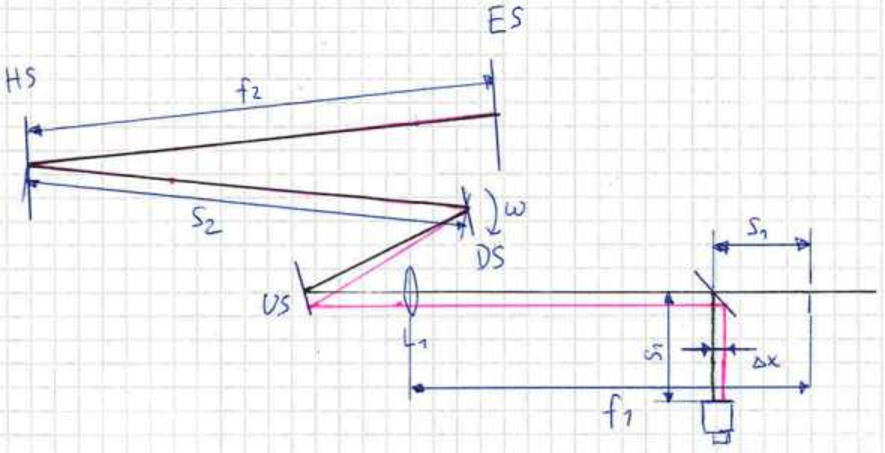
\includegraphics[width=\textwidth]{images/setup.pdf}
    \caption{}
    \label{fig:setup}
\end{figure}

Die Distanz $S_1$ vom Laserstrahl zum Okular wird gemessen und der Spalt wird
verschoben, bis er auch mit der Distanz $S_1$ vom Strahlteiler entfernt ist.

Gemessen wurde $S_1 = (107\pm3)\textrm{mm}$.

Jetzt  wird die  Linse $L_1$  in den  Laserstrahl eingef\"ugt. Die  Linse muss
gleich der Brennweite $f_1 = 1000\textrm{mm}$ vom Spalt distanziert werden.

Gemessen wurde die Distanz von der Linse $L_1$ zum Spalt $(998\pm3)\textrm{mm}$.

\begin{figure}[H]
    \center
    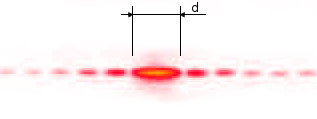
\includegraphics[width=.9\textwidth]{images/diffraction.png}
    \caption{}
    \label{fig:diffraction}
\end{figure}


\subsection{Messvorgang}

\subsection{Messungen}


